\appendix
\section{Variational Free Energy Derivation}
\label{app:vfe-derivation}

This appendix gives the algebraic derivation used to motivate the variational free energy objective in Sect.~\ref{subsec:first-principles}. Let $x$ denote hidden state, $y$ denote observations, and $q(x;\zeta)$ denote an approximate posterior belief parameterized by $\zeta$. The Kullback--Leibler divergence between $q(x;\zeta)$ and the true posterior $p(x\mid y)$ is
\begin{equation}
    D_{\mathrm{KL}}
    \left(
        q(x;\zeta) \,\|\, p(x\mid y)
    \right)
    =
    \int q(x;\zeta)
    \ln
    \left(
        \frac{q(x;\zeta)}{p(x\mid y)}
    \right) dx .
    \label{eq:appendix-kl-posterior}
\end{equation}
Using Bayes' rule, $p(x\mid y)=p(x,y)/p(y)$, gives
\begin{align}
    D_{\mathrm{KL}}
    \left(
        q(x;\zeta) \,\|\, p(x\mid y)
    \right)
    &=
    \int q(x;\zeta)
    \ln
    \left(
        \frac{q(x;\zeta)p(y)}{p(x,y)}
    \right) dx
    \nonumber \\
    &=
    \int q(x;\zeta)
    \ln
    \left(
        \frac{q(x;\zeta)}{p(x,y)}
    \right) dx
    +
    \int q(x;\zeta)\ln p(y)\,dx .
    \label{eq:appendix-kl-expanded}
\end{align}
Because $\ln p(y)$ does not depend on $x$, and the integral over a probability density $q(x;\zeta)$ integrates to one, this becomes
\begin{equation}
    D_{\mathrm{KL}}
    \left(
        q(x;\zeta) \,\|\, p(x\mid y)
    \right)
    =
    \underbrace{
    \int q(x;\zeta)
    \ln
    \left(
        \frac{q(x;\zeta)}{p(x,y)}
    \right) dx
    }_{\mathcal{F}(y,\zeta)}
    +
    \ln p(y).
    \label{eq:appendix-vfe-definition}
\end{equation}
The bracketed term is variational free energy:
\begin{equation}
    \mathcal{F}(y,\zeta)
    =
    \int q(x;\zeta)
    \ln
    \left(
        \frac{q(x;\zeta)}{p(x,y)}
    \right) dx .
    \label{eq:appendix-vfe}
\end{equation}
Since $\ln p(y)$ is independent of the variational parameters $\zeta$, minimizing $\mathcal{F}(y,\zeta)$ with respect to $\zeta$ is equivalent to minimizing the KL divergence between the approximate belief and the true posterior.

\section{Laplace-Encoded Free Energy Approximation}
\label{app:laplace-free-energy}

The full derivation is given by Buckley et al.~\cite{buckley_free_2017}. Here we outline the key steps for the univariate case, using the notation of this paper, to explain how variational free energy leads to precision-weighted prediction-error minimization.
\\


Starting from the variational free energy definition,
\begin{equation}
    \mathcal{F}(y,\zeta)
    =
    \int q(x;\zeta)
    \ln
    \left(
        \frac{q(x;\zeta)}{p(x,y)}
    \right) dx ,
\end{equation}
and using $\ln(a/b)=\ln(a)-\ln(b)$, and defining the Laplace-encoded energy as
\begin{equation}
    E(x,y)=-\ln p(x,y).
\end{equation}
This gives
\begin{equation}
    \mathcal{F}(y,\zeta)
    =
    \int q(x;\zeta)E(x,y)\,dx
    +
    \int q(x;\zeta)\ln q(x;\zeta)\,dx .
    \label{eq:appendix-laplace-energy}
\end{equation}
Under the Laplace assumption, the recognition density is approximated as a sharply peaked Gaussian around its mean $\mu$:
\begin{equation}
    q(x;\zeta)
    =
    \frac{1}{\sqrt{2\pi\sigma^2}}
    \exp
    \left(
        -\frac{(x-\mu)^2}{2\sigma^2}
    \right).
\end{equation}
Substituting this Gaussian into Eq.~\ref{eq:appendix-laplace-energy} yields
\begin{equation}
    \mathcal{F}(y,\zeta)
    =
    \int q(x;\zeta)E(x,y)\,dx
    -
    \ln\sqrt{2\pi\sigma^2}
    -
    \frac{1}{2}.
\end{equation}

Applying a second-order Taylor approximation to $E(x,y)$ around
$x=\mu$, where the Gaussian density is concentrated, allows us
to rewrite the approximation as (note: first order derivative is 0 because sharply peaked at $\mu$):
\begin{equation}
    \mathcal{F}(y,\zeta)
    \approx E(\mu,y)
    + \frac{1}{2}\left(
        \left.\frac{d^2E}{dx^2}\right|_{\mu}\sigma^2
        - \ln(2\pi\sigma^2)-1
    \right).
\end{equation}


By solving $\partial\mathcal{F}/\partial\sigma^2=0$ with respect
to the variance $\sigma^2$, which optimizes the free energy,
this further simplifies to
\begin{equation}
    \mathcal{F}(y,\zeta)
    \approx E(\mu,y)-\frac{1}{2}\ln(2\pi\sigma^{2*}),
\end{equation}

where $\sigma^{2*}=\left[\left.d^2E/dx^2\right|_{\mu}\right]^{-1}$
is the variance that optimizes the free energy. It is calculated
from the local curvature at the mean $\mu$. In other words, the
free energy only depends on the Gaussian mean $\mu$ and not on
an independent variance $\sigma^2$, which simplifies the expression.
To simplify further, we treat the variance correction as constant
during mean updating. Since the objective is to minimize free
energy, this constant can be omitted. The Laplace-encoded free
energy approximation is then written as

\begin{equation}
    \mathcal{F}(y,\zeta)\approx E(\mu,y)=-\ln p(\mu,y).
\end{equation}
\\
For the robot-localization case, the joint probability can be written as a likelihood times a prior-like motion term:
\begin{equation}
    p(\mu,y)
    =
    p(y\mid\mu)p(\mu).
\end{equation}
Therefore,
\begin{align}
    \mathcal{F}(y,\mu)
    &=
    -\ln p(\mu,y)
    \nonumber \\
    &=
    -\ln\left(p(y\mid\mu)p(\mu)\right)
    \nonumber \\
    &=
    -\ln p(y\mid\mu)
    -
    \ln p(\mu).
\end{align}
With Gaussian sensory and motion prediction errors,
\begin{align}
    p(y\mid\mu)
    &=
    \frac{1}{\sqrt{2\pi\sigma_z^2}}
    \exp
    \left(
        -\frac{\left(y-g(\mu)\right)^2}{2\sigma_z^2}
    \right),
    \nonumber \\
    p(\mu)
    &=
    \frac{1}{\sqrt{2\pi\sigma_w^2}}
    \exp
    \left(
        -\frac{\left(\mu-f(\mu)\right)^2}{2\sigma_w^2}
    \right).
\end{align}
Substituting these densities and using $\ln(e^a)=a$, and $\ln(\sqrt{a})=\frac{1}{2}\ln(a)$ gives
\begin{align}
    \mathcal{F}(y,\mu)
    &=
    \frac{\left(y-g(\mu)\right)^2}{2\sigma_z^2}
    +
    \frac{\left(\mu-f(\mu)\right)^2}{2\sigma_w^2}
    +
    \frac{1}{2}\ln\left(\sigma_z^2\sigma_w^2\right)
    +
    \ln(2\pi).
\end{align}
The final term is constant with respect to the belief mean and can be omitted for belief updating. Defining prediction errors
\begin{equation}
    \epsilon_z = y-g(\mu),
    \qquad
    \epsilon_w = \mu-f(\mu),
\end{equation}
and precisions $\Pi_z=1/\sigma_z^2$ and $\Pi_w=1/\sigma_w^2$ yields
\begin{equation}
    \mathcal{F}(y,\mu)
    \approx
    \frac{1}{2}\Pi_z\epsilon_z^2
    +
    \frac{1}{2}\Pi_w\epsilon_w^2
    -
    \frac{1}{2}\ln\left(\Pi_z\Pi_w\right).
\end{equation}


\section{Derivation of the Generalized-Coordinate Update}
\label{app:slide15-update-derivation}

The generalized-coordinate update can be written as
\begin{equation}
    \dot{\tilde{\mu}}_{g}
    -
    D\tilde{\mu}_{g}
    =
    -
    \partial_{\tilde\mu_g}\mathcal{F}(y,\mu).
    \label{eq:appendix-slide15-gradient-balance}
\end{equation}
The term $D\tilde{\mu}_{g}$ is due to the generalized coordinates. When the true motion equals the belief of the motion, $\dot{\tilde{\mu}}_{g}=D\tilde{\mu}_{g}$, the free-energy gradient should reach zero: $\dot{\tilde{\mu}}_{g}-D\tilde{\mu}_{g}=-\partial_{\mu_g}\mathcal{F}=0$.

Which can be rewritten as:
\begin{equation}
    \dot{\tilde{\mu}}_{g}
    =
    D\tilde{\mu}_{g}
    -
    \partial_{\tilde\mu_g}\mathcal{F}(y,\mu).
    \label{eq:appendix-slide15-start}
\end{equation}
 Substituting the Free Energy terms with constants, and the respective error terms in equation \ref{eq:prediction-errors}, gives
\begin{align}
    \dot{\tilde{\mu}}_{g}
    &=
    D\tilde{\mu}_{g}
    -
    \left(
        \partial_{\tilde\mu_g}\tilde{\epsilon}_{g}^{\top}
        \tilde{\Pi}_{g}\tilde{\epsilon}_{g}
        +
        \partial_{\tilde\mu_g}
        \sum_{\mathrm{landmarks}}
        \left(
            \tilde{\epsilon}_{p}^{\top}
            \tilde{\Pi}_{p}\tilde{\epsilon}_{p}
        \right)
    \right)
    \nonumber \\
    &=
    D\tilde{\mu}_{g}
    -
    \left(
        D
        -
        \partial_{\tilde\mu_g}\tilde{f}(\tilde{\mu}_{g})
    \right)^\top
    \tilde{\Pi}_{g}\tilde{\epsilon}_{g}
    +
    \sum_{\mathrm{landmarks}}
    \left(
        \partial_{\tilde\mu_g}\tilde{g}(\tilde{\mu}_{g})
    \right)^\top
    \tilde{\Pi}_{p}\tilde{\epsilon}_{p}
    \nonumber \\
    &=
    D\tilde{\mu}_{g}
    -
    D^\top\tilde{\Pi}_{g}\tilde{\epsilon}_{g}
    +
    \left(
        \partial_{\tilde\mu_g}\tilde{f}(\tilde{\mu}_{g})
    \right)^\top
    \tilde{\Pi}_{g}\tilde{\epsilon}_{g}
    +
    \sum_{\mathrm{landmarks}}
    \left(
        \partial_{\tilde\mu_g}\tilde{g}(\tilde{\mu}_{g})
    \right)^\top
    \tilde{\Pi}_{p}\tilde{\epsilon}_{p}.
    \tag{\ref{eq:slide15-generic-update}}
    \label{eq:appendix-slide15-derivation}
\end{align}
The continuous belief dynamics are then integrated with the forward Euler method:
\begin{equation}
    \tilde{\mu}_{g}(t+\Delta t)
    =
    \tilde{\mu}_{g}(t)
    +
    \Delta t\,
    \dot{\tilde{\mu}}_{g}(t).
    \label{eq:appendix-slide15-euler}
\end{equation}

\section{Coordinate System Conventions}
\label{app:coordinate-conventions}

The coordinate conventions follow the ROS 2 convention defined by REP 103~\cite{ros_rep_103}. ROS 2 is a widely used robotics middleware that standardizes how robot software components exchange sensor data, poses, velocities, and coordinate-frame transformations. REP 103 defines common coordinate-frame conventions for interoperability; for robot body frames, $+X$ points forward, $+Y$ points left, and $+Z$ points up. We use two planar coordinate systems throughout the paper: the Field Coordinate System (FCS), which is fixed to the soccer field, and the Robot Coordinate System (RCS), which is fixed to the robot.

\begin{figure}[htbp]
    \centering
    \begin{minipage}[t]{0.32\textwidth}
        \centering
        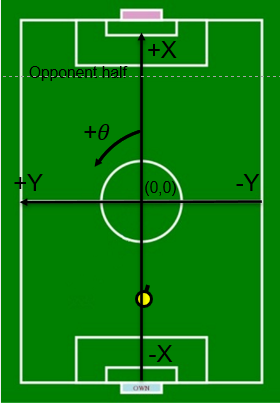
\includegraphics[width=\linewidth]{figures/FCS_field_view.png}
        \small (a) Field Coordinate System (FCS).
    \end{minipage}
    \hspace{0.05\textwidth}
    \begin{minipage}[t]{0.42\textwidth}
        \centering
        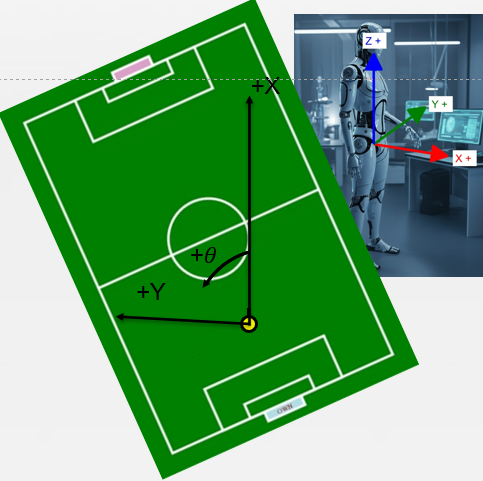
\includegraphics[width=\linewidth]{figures/RCS_field_view.png}
        \small (b) Robot Coordinate System (RCS).
    \end{minipage}
    \caption{Coordinate systems used in the paper. In FCS, the origin is the center of the field, $+X$ points toward the opponent goal, $+Y$ points left, and $\theta=0$ rad points toward the opponent goal. In RCS, the origin is the robot center, $+X$ points forward from the robot perspective, $+Y$ points to the robot's left, and $\theta=0$ rad points straight forward.}
    \label{fig:appendix-coordinate-systems}
\end{figure}

In FCS, robot pose and known landmark positions are expressed in field coordinates. The point $(0,0)$ is the center point of the field. The $+X$ direction points toward the opponent goal, and $+Y$ points to the left. The orientation angle $\theta$ is expressed in radians; $\theta=0$ points toward the opponent goal, and positive rotation is toward the left.

In RCS, observations are expressed from the robot's perspective. The origin is the center of the robot. The $+X$ direction points forward, and $+Y$ points to the robot's left. The angle convention is again in radians, with $\theta=0$ straight ahead and positive rotation toward the left. 

With these conventions, the RCS-to-FCS translation used for motion observations is
\begin{equation}
    \begin{bmatrix}
        v_x^{\mathrm{FCS}} \\
        v_y^{\mathrm{FCS}} \\
        \omega^{\mathrm{FCS}}
    \end{bmatrix}
    =
    \begin{bmatrix}
        \cos\theta_r & -\sin\theta_r & 0 \\
        \sin\theta_r & \cos\theta_r & 0 \\
        0 & 0 & 1
    \end{bmatrix}
    \begin{bmatrix}
        v_x^{\mathrm{RCS}} \\
        v_y^{\mathrm{RCS}} \\
        \omega^{\mathrm{RCS}}
    \end{bmatrix}.
    \label{eq:fcs-rcs-motion-transform}
\end{equation}

The landmark observation model translates a candidate robot pose in FCS and a known landmark position in FCS into the expected landmark observation in RCS. The inputs are
\begin{equation}
    \mathrm{robot}_{\mathrm{FCS}}
    =
    \begin{bmatrix}
        x_r \\
        y_r \\
        \theta_r
    \end{bmatrix},
    \qquad
    \ell_{\mathrm{FCS}}
    =
    \begin{bmatrix}
        x_l \\
        y_l
    \end{bmatrix}.
    \label{eq:landmark-inputs-fcs}
\end{equation}

The corresponding FCS-to-RCS landmark prediction is
\begin{equation}
    \begin{bmatrix}
        x_{pl} \\
        y_{pl} \\
        \theta_{pl}
    \end{bmatrix}
    =
    \begin{bmatrix}
        \cos\theta_r (x_l-x_r) + \sin\theta_r (y_l-y_r) \\
        -\sin\theta_r (x_l-x_r) + \cos\theta_r (y_l-y_r) \\
        \operatorname{atan2}(y_{pl},x_{pl})
    \end{bmatrix}.
    \label{eq:fcs-to-rcs}
\end{equation}

Because the soccer field and coordinate conventions are known, the corresponding landmark Jacobian with respect to the pose components $(x_r,y_r,\theta_r)$ is calculated directly as
\begin{equation}
    J_\ell
    =
    \begin{bmatrix}
        -\cos\theta_r & -\sin\theta_r & y_{pl} \\
        \sin\theta_r & -\cos\theta_r & -x_{pl} \\
        \dfrac{y_l-y_r}{(x_l-x_r)^2+(y_l-y_r)^2}
        &
        -\dfrac{x_l-x_r}{(x_l-x_r)^2+(y_l-y_r)^2}
        &
        -1
    \end{bmatrix}.
    \label{eq:landmark-jacobian}
\end{equation}
This Jacobian is the term $\partial_{\mu_g}\tilde{g}(\tilde{\mu}_g)$ in Eq.~\ref{eq:slide15-generic-update}. It propagates landmark prediction errors back to the field-pose belief.

To clarify, $x_r$, $y_r$, and $\theta_r$ are the current belief
estimates of the robot pose; all transformations and the Jacobian
above are evaluated using these estimates, without access to the
actual robot pose.

\FloatBarrier

\section{Tracking Error for Different Landmark Configurations}
\label{sec:appendix-landmark-tracking}

This appendix provides a more detailed view of the tracking behavior evaluated in Section~\ref{subsec:experiments-visibility-stress}, how landmark availability affects tracking
error over time. 


\begin{figure}[htbp]
    \centering

    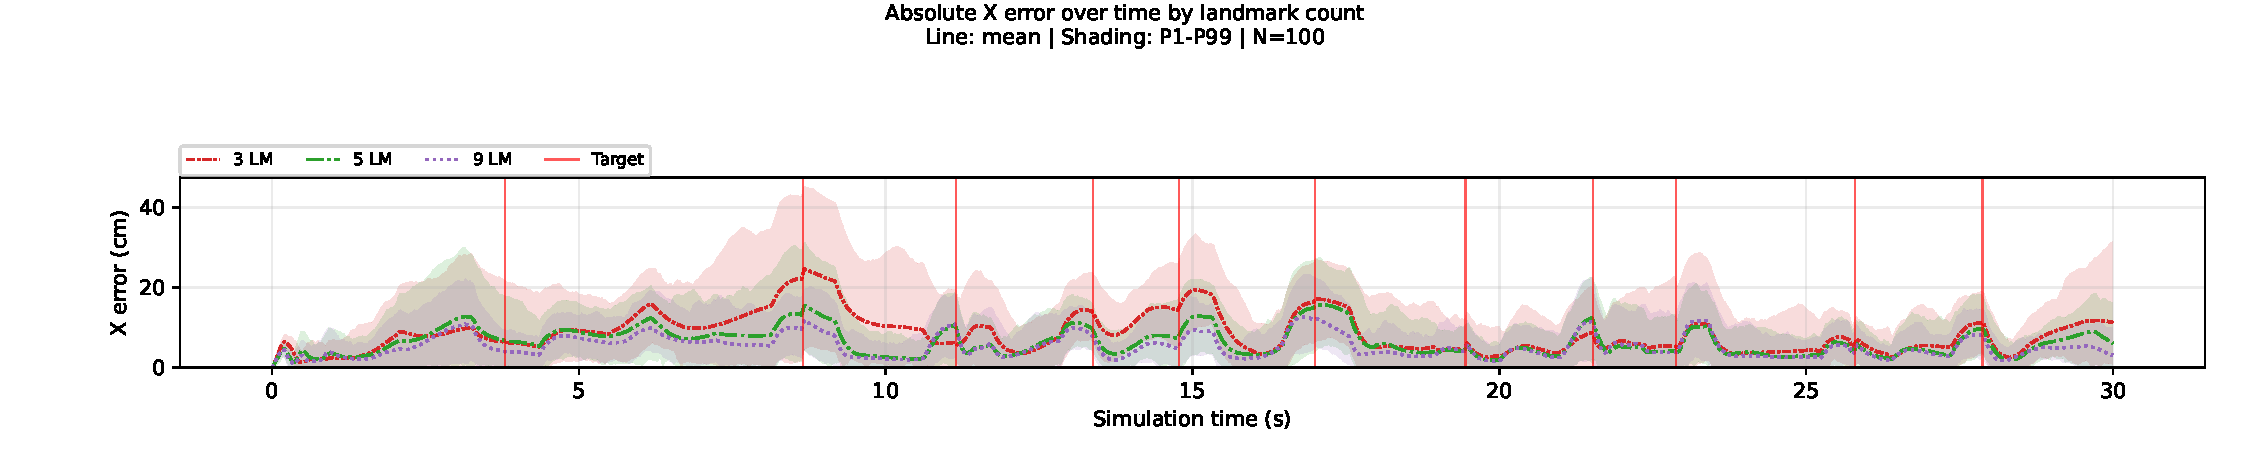
\includegraphics[width=\linewidth,page=1]
    {figures/paper_lm_dataset_20260918_111044_227495_graph.pdf}\\
    {\small (a) Absolute $x$-position error}

    \medskip

    \includegraphics[width=\linewidth,page=2]
    {figures/paper_lm_dataset_20260918_111044_227495_graph.pdf}\\
    {\small (b) Absolute $y$-position error}

    \medskip

    \includegraphics[width=\linewidth,page=3]
    {figures/paper_lm_dataset_20260918_111044_227495_graph.pdf}\\
    {\small (c) Absolute heading error}

    \caption{\scriptsize
    Each landmark configuration (3: two goals and the middle circle; 5: additionally, the two halfway-line boundary points; 9: additionally, the four corners) is evaluated over 100 trials of 30 seconds. All 100 trials for every landmark configuration use identical initial actual and belief poses and replay the same randomly generated target sequence. The trials use the same noise, dropout, field-of-view, and temporary-obstruction settings as Section~\ref{subsec:experiments-visibility-stress}. Landmark counts describe the available map; the number observed at each timestep may be smaller due to the 110 degrees field-of-view. Panels show absolute errors in (a) $x$ position, (b) $y$ position, and (c) heading. Lines show the mean absolute belief-minus-actual error across trials at each timestep; shaded regions span the 1st to 99th percentiles. Heading error is the absolute wrapped angular difference. Thin red vertical lines indicate activation of the next random target.}
    \label{fig:landmark-tracking-error}
\end{figure}
\FloatBarrier